\documentclass{standalone}
\usepackage{tikz}
\usetikzlibrary{arrows,shapes,positioning,shadows,trees}

\begin{document}
\begin{tikzpicture}
    \draw[-] (-3,0) -- (5,0);
    \node[fill,circle,inner sep=1pt,label=below:$O$] at (0,0) {};
    \draw[->] (4,0.2) arc (0:185:3);
    \draw[->] (-2,0) arc (180:355:3);
    \draw[<-] (1,0.2) arc (10:180:1);
    \draw[<-] (-1,0) arc (180:350:1);

    \node[fill,circle,inner sep=1pt,label=below:$-1$] at (-1.5,0) {};
    \node[fill,circle,inner sep=1pt,label=above right:$R$] at (4,0) {};
    \draw[->] (1,0.2) -- (4,0.2);
    \draw[<-] (1,-0.2) -- (4,-0.2);
\end{tikzpicture}

\begin{tikzpicture}
    \node[fill,circle,inner sep=1pt,label=below:$O$] at (0,0) {};
    \draw[<-] (1,0) arc (0:180:1);
    \draw[->] (1,0) -- (4,0);
    \draw[<-] (-1,0) -- (-4,0);
    \draw[<-] (4,0) arc (0:180:4);
    \node[fill,circle,inner sep=1pt,label=below:$-\rho$] at (-1,0) {};
    \node[fill,circle,inner sep=1pt,label=below:$\rho$] at (1,0) {};
    \node[fill,circle,inner sep=1pt,label=below:$-R$] at (-4,0) {};
    \node[fill,circle,inner sep=1pt,label=below:$R$] at (4,0) {};
    \node[label=above right:$\gamma_R$] at (4 * 0.6,4 * 0.8) {};
    \node[label=above right:$\gamma_\rho$] at (1 * 0.6,1 * 0.8) {};
    \node[fill,circle,inner sep=1pt,label=right:$i$] at (0,2.5) {};
\end{tikzpicture}


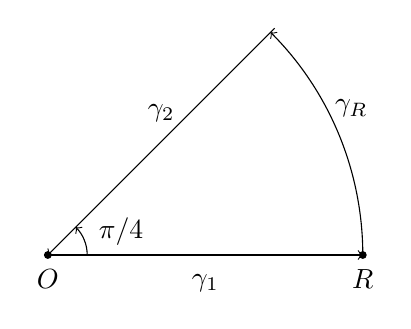
\begin{tikzpicture}
    \draw[->] (0,0) -- (4,0);
    \node[fill,circle,inner sep=1pt,label=below:$O$] at (0,0) {};
    \node[fill,circle,inner sep=1pt,label=below:$R$] at (4,0) {};
    \node[label=below:$\gamma_1$] at (2,0) {};
    \draw[->] (4,0) arc (0:45:4);
    \node[label=above right:$\gamma_R$] at (3.4, 1.5) {};
    \draw[->] (4 * 0.72,4*0.72) -- (0,0);
    \node[label=above:$\gamma_2$] at (2 * 0.72, 2 * 0.72) {};
    \draw[->] (0.5,0) arc (0:45:0.5);
    \node[label=right:$\pi/4$] at (0.5 * 0.8, 0.5 * 0.6) {};
\end{tikzpicture}

\begin{tikzpicture}
    \draw[-] (-4,0) -- (4,0);
    \node[fill,circle,inner sep=1pt,label=below:$O$] at (0,0) {};
    \node[fill,circle,inner sep=1pt,label=below:$-R$] at (-3,0) {};
    \node[fill,circle,inner sep=1pt,label=below:$R$] at (3,0) {};
    \draw[->] (0,0) -- (0,2.5);
    \draw[->] (3,0) -- (3,1);
    \draw[-] (3,1) -- (3,2);
    \node[label=above right:$\gamma_1$] at (3,1) {};
    \draw[->] (3,2) -- (2,2);
    \draw[-] (2,2) -- (-3,2);
    \node[label=above right:$\gamma_2$] at (2,2) {};
    \draw[->] (-3,2) -- (-3,1);
    \draw[-] (-3,1) -- (-3,0);
    \node[label=above left:$\gamma_3$] at (-3,1) {};
    \node[label=above right:$R+\frac{b}{2a}i$] at (3,2) {};
\end{tikzpicture}
\end{document}